%!TEX TS-program = xelatex

%%%%%%%%%%%%%%%%%%%%%%%%%%%%%%%%%%%%%%%%%%%%%%%%
% CV template
% Originally created by Adrien Friggeri
% Improved by Carmine Benedetto
%%%%%%%%%%%%%%%%%%%%%%%%%%%%%%%%%%%%%%%%%%%%%%%%

\documentclass[]{cv-class}
\usepackage{afterpage}
\usepackage{hyperref}
\usepackage{color}
\usepackage{xcolor}
\hypersetup{
    colorlinks=true,
    linkcolor=blue
}
\addbibresource{bibliography.bib}
\RequirePackage{xcolor}
\definecolor{pblue}{HTML}{0395DE}

\begin{document}
\header{Martin}{Othamar}
      {developer}
      
% Fake text to add separator    
\vspace{1.15cm}  
\fcolorbox{white}{gray}{\parbox{\dimexpr\textwidth-2\fboxsep-2\fboxrule}{%
.....
}}

% In the aside, each new line forces a line break
\begin{aside}
  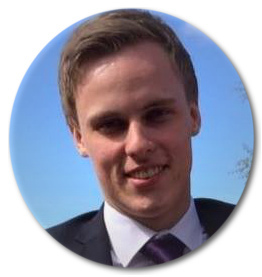
\includegraphics[scale=0.40]{img/meg2.jpg}
  	~
  \section{Address}
    Trollkleiva, 8
    4638, Kristiansand, Norway
    ~
  \section{Phone}
    +47 47 35 60 90
    ~
  \section{Mail}
    \underline{\href{mailto:martin@othamar.net}{martin@othamar.net}}
    ~
  \section{Web \& Git}
  	\underline{\href{http://martinothamar.github.io}{martinothamar.github.io}}
    \underline{\href{https://no.linkedin.com/in/martinothamar}{linkedin.com/in/martinothamar}}
    \underline{\href{https://github.com/martinothamar}{github.com/martinothamar}}
    ~
  \section{Programming}
    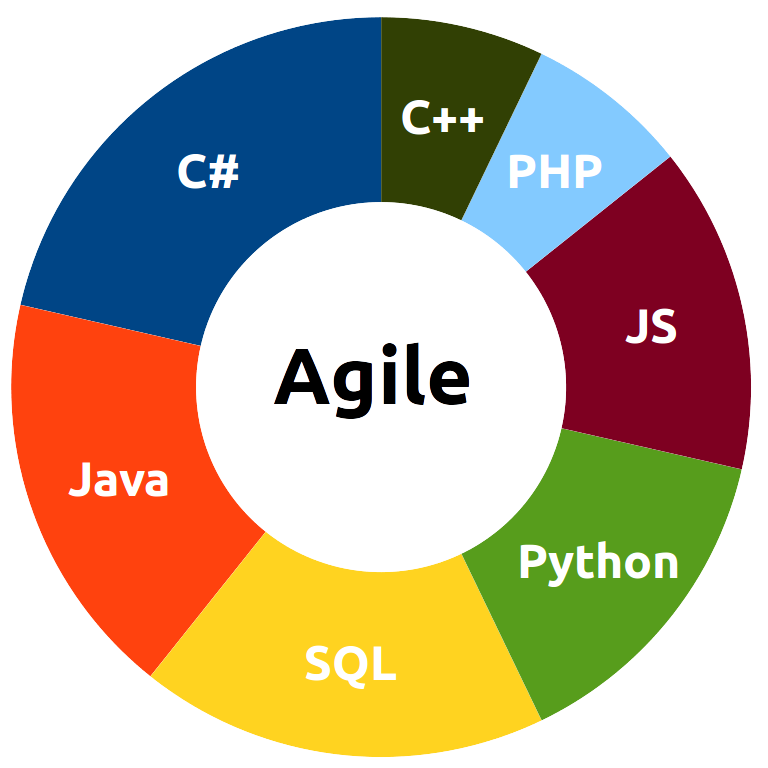
\includegraphics[scale=0.22]{img/programming2.png}
    ~

  \section{Personal Skills}
    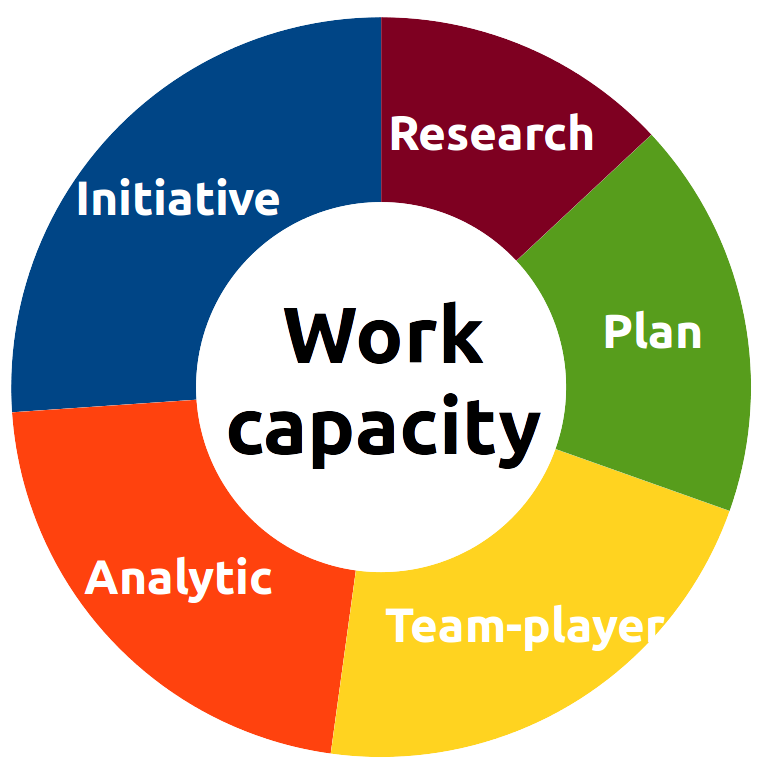
\includegraphics[scale=0.22]{img/personal2.png}
    ~
  \section{OS Preference}
    \asidelist{\textbf{Linux}}
    {
\includegraphics[scale=0.30]{img/star.png}
    
\includegraphics[scale=0.30]{img/star.png}
    
\includegraphics[scale=0.30]{img/star.png}
    
\includegraphics[scale=0.30]{img/star.png}
    
\includegraphics[scale=0.30]{img/star.png}}
    \asidelist{\textbf{Windows}}
    {
\includegraphics[scale=0.30]{img/star.png}
    
\includegraphics[scale=0.30]{img/star.png}
    
\includegraphics[scale=0.30]{img/star.png}
    
\includegraphics[scale=0.30]{img/star.png}
    
\includegraphics[scale=0.30]{img/star_empty.png}}
    ~
\end{aside}

\vspace{0.75cm}
\section{Experience}
\begin{entrylist}
  \entry
    {Sept. 15 - Now}
    {Co-Founder \& IT Consultant}
    {EnterCon DA, Kristiansand/Oslo}
    {Delivering web sites, apps and marketing solutions to businesses
    in southern and eastern Norway. I am responsible for development,
    hosting and internal IT infrastructure like website, ERP (Odoo) etc.\\}
  \entry
    {Aug. 15 - Now}
    {Software Developer}
    {meQuire Solutions AS, Kristiansand}
    {Back end development on a software-stack consisting of the following 
    technologies NodeJS, HAPI, RethinkDB using Amazon Web Services hosting.\\}
  \entry
    {Aug. 15 - Now}
    {Teaching Assistant}
    {University of Agder, Kristiansand}
    {Helping third year students in the IT and Information Systems Bachelor's degree programme
    learn in IS-213: Open Source Development.\\}
  \entry
    {Jan. 15 - May 15}
    {Bachelor thesis - IS-304}
    {Frontica Business Solutions, Kristiansand}
    {Full stack development and full remake/modernization of legacy Information Quality system
    on the .NET platform with C\# with technologies like ASP.NET Web Api 2,
    MVC, Windows Service, WCF, 
    Twitter Bootstrap front end with JS/jQuery. Worked agile with Scrum on TFS 2012 /w TFVC
    and BDD for testing.
    \emph{Title of the Thesis: 
    "The Reengineering of Frontica Business Solutions' Information Quality System".} 
    Grade: \textbf{A}.\\}
  \entry
    {Sept. 14 - Dec. 14}
    {Internship - IS-302}
    {Frontica Business Solutions, Kristiansand}
    {Documentation of in-house VBA application as well as full stack development of 
    in-house Active Directory
    user information reporting service on the .NET platform with C\#. ASP.NET MVC, 
    QUARTZ.NET for scheduled jobs
    and Twitter Bootstrap, JS/jQuery on the front end. Grade: \textbf{A}.\\}
\end{entrylist}


\section{Education}
\begin{entrylist}
  \entry
    {Aug. 15 - Now}
    {Master's Degree (MSc) in Information Systems}
    {University of Agder}
    {Information Systems Master's Degree focusing on Systems Development
    /Software Engineering, Enterprise Systems (ERP), Business Development and 
    IT Project Management.\\}
  \entry
    {Aug. 13 - June 15}
    {Bachelor's Degree (BSc) in IT and Information Systems}
    {University of Agder}
    {An IT and Information Systems education focused on the interdisciplinarity of
    systems development and project/business management subjects.\\
    \emph{Title of the Thesis: "The Reengineering of Frontica Business Solutions' 
    Information Quality System". Grade \textbf{A}}.\\}
  \entry
    {Aug. 09 - June 12}
    {University Admissions Certification}
    {Toppidrettsgymnaset i Telemark}
    {Top-level Sports Upper secondary school.
    Main subjects: Football (soccer), International English, Sociology and Social Anthropology,
    Politics and Human Rights, Social Studies English.}
\end{entrylist}



\newpage
\begin{aside}
  \section{Places lived}
    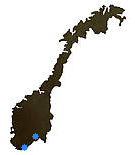
\includegraphics[scale=0.62]{img/norway.png}
    ~
  \section{Languages}
    \asidelist{\textbf{Norwegian}}
    {
\includegraphics[scale=0.30]{img/star.png}
    
\includegraphics[scale=0.30]{img/star.png}
    
\includegraphics[scale=0.30]{img/star.png}
    
\includegraphics[scale=0.30]{img/star.png}
    
\includegraphics[scale=0.30]{img/star.png}}
    \asidelist{\textbf{English}}
    {
\includegraphics[scale=0.30]{img/star.png}
    
\includegraphics[scale=0.30]{img/star.png}
    
\includegraphics[scale=0.30]{img/star.png}
    
\includegraphics[scale=0.30]{img/star.png}
    
\includegraphics[scale=0.30]{img/star_empty.png}}
    \asidelist{\textbf{Faroese}}
    {
\includegraphics[scale=0.30]{img/star.png}
    
\includegraphics[scale=0.30]{img/star.png}
    
\includegraphics[scale=0.30]{img/star_empty.png}
    
\includegraphics[scale=0.30]{img/star_empty.png}
    
\includegraphics[scale=0.30]{img/star_empty.png}}
    \asidelist{\textbf{German}}
    {
\includegraphics[scale=0.30]{img/star.png}
    
\includegraphics[scale=0.30]{img/star_empty.png}
    
\includegraphics[scale=0.30]{img/star_empty.png}
    
\includegraphics[scale=0.30]{img/star_empty.png}
    
\includegraphics[scale=0.30]{img/star_empty.png}}
    ~
\end{aside}



\section{Projects}
\begin{entrylist}
  \entry
    {Aug. 15 - Now}
    {UiA Schedule for Android}
    {EnterCon project}
    {An Android application for displaying the schedule is a user-friendly,
    mobile-friendly manner. The scraping-logic from the C\# Schedule Scraper below
    was ported to Java so that the app runs natively.
    \underline{\href{https://github.com/martinothamar/UiA-Timeplan-Android}
    {Github repository}}.\\}
  \entry
    {June 15}
    {UiA Schedule Scraper}
    {Solo project}
    {A C\# console application scraping university programme schedule information
    of their webpage, outputting JSON.
    \underline{\href{https://github.com/martinothamar/UiA-ScheduleGrabber}
    {Github repository}}.\\}
  \entry
    {Aug. 14 - Dec. 14}
    {Slit.nu}
    {University of Agder}
    {Portal for module based learning, written in Java with JSF, OpenJPA on a TomEE server.
    Developed in the course of IS-202: Programming project.\\}
  \entry
    {Jan. 14 - Feb. 14}
    {NetworkIT}
    {Solo project}
    {Web-based recruitment platform.
    Built on the LAMP-stack with Laravel and Twitter Bootstrap + jQuery for the front end.
    \underline{\href{https://bitbucket.org/martinothamar/networkit}{Bitbucket repository}}.\\}
  \entry
    {Sept. 13 - Jan. 14}
    {Nettverket-SB}
    {Student company, {{\O}}stfold University College}
    {Career portal for newly educated and students.
    Built on the LAMP-stack with a homemade MVC framework and 
    Twitter Bootstrap + jQuery for the front end.
    \underline{\href{https://github.com/martinothamar/Nettverket-SB}{Github repository}}.}
\end{entrylist}


\section{Certifications}
\begin{entrylist}
  \entry
    {Oct. 15}
    {PRINCE2 Foundation certification}
    {University of Agder, Kristiansand}
    {Foundation-level Project Management certification.}
\end{entrylist}

\vspace{1.5cm}
\begin{flushright}
\emph{Martin Othamar}
\end{flushright}
\begin{flushright}
\emph{\today}
\end{flushright}

\end{document}
